\documentclass[aspectratio=169]{beamer}
\usepackage[utf8]{inputenc}
\usepackage[T1]{fontenc}
\usepackage[spanish]{babel}
\usepackage{graphicx}
\usepackage{booktabs}
\usepackage{xcolor}
\usepackage{colortbl}
\usepackage{tikz}
\usepackage{pgfplots}
\pgfplotsset{compat=1.18}
\usetikzlibrary{shapes.geometric, arrows.meta, positioning, calc}

\usetheme{Madrid}
\usecolortheme{seahorse}
\setbeamertemplate{navigation symbols}{}
\setbeamertemplate{footline}[frame number]

% Colores corporativos
\definecolor{verdebueno}{RGB}{46, 125, 50}
\definecolor{amarillomedio}{RGB}{245, 124, 0}
\definecolor{rojomalo}{RGB}{183, 28, 28}
\definecolor{azulinst}{RGB}{18, 56, 95}

% Logo institucional (arriba izquierda, pequeño y centrado en la franja blanca)
\setbeamertemplate{headline}{%
  \parbox[c][0.9cm][c]{\paperwidth}{%
    \hspace{0.4cm}%
    
\includegraphics[height=0.45cm]{logo_oficina.jpg}%
    \hfill%
  }%
}

% Aplicar color corporativo a estructura de Beamer
\setbeamercolor{structure}{fg=azulinst}
\setbeamercolor{frametitle}{fg=white,bg=azulinst}
\setbeamercolor{title}{fg=white,bg=azulinst}

\newcommand{\cmarks}{\textcolor{verdebueno}{\checkmark}}
\newcommand{\xmark}{\textcolor{rojomalo}{$\times$}}

\title{Evaluaci\'{o}n comparativa de alternativas de tratamiento}
\subtitle{PTAR Puerto Baquerizo Moreno \textbullet{} Gal\'{a}pagos}
\author{Equipo t\'{e}cnico}
\date{Caudal de dise\~{n}o: 17.31~L/s \textbullet{} 3 l\'{i}neas paralelas}
\institute{Informe t\'{e}cnico comparativo}

\begin{document}

% ========================================================================
% DIAPO 1: PORTADA
% ========================================================================
\begin{frame}
\titlepage
\end{frame}





% ========================================================================
% DIAPO 2: CONTEXTO EN TIKZ
% ========================================================================
\begin{frame}
\frametitle{Contexto: el tren actual y la propuesta con lodos activados}
\centering
\begin{tikzpicture}[
    scale=0.7, transform shape,
    box/.style={rectangle, rounded corners=6pt, draw=black, line width=1pt, minimum width=5cm, minimum height=0.7cm, align=center, font=\footnotesize},
    arrow/.style={->, >=stealth, line width=1pt},
    title/.style={font=\bfseries\small}
]
% ==========================================
% IZQUIERDA: TREN ACTUAL
% ==========================================
\node[title] (ta) at (-3.3, 0.3) {TREN ACTUAL DE LA PTAR};
\node[box, below=0.2cm of ta] (a1) {Afluente crudo};
\node[box, below=0.3cm of a1] (a2) {Pre-sedimentador};
\node[box, below=0.3cm of a2] (a3) {Filtro anaerobio\\de flujo ascendente};
\node[box, below=0.3cm of a3] (a4) {Tanques de aireaci\'{o}n};
\node[box, below=0.3cm of a4] (a5) {Filtro percolador};
\node[box, below=0.3cm of a5] (a6) {Coagulaci\'{o}n - floculaci\'{o}n};
\node[box, below=0.3cm of a6] (a7) {Filtros de carb\'{o}n activado};
\node[box, below=0.3cm of a7] (a8) {Cloraci\'{o}n / desinfecci\'{o}n\\$\rightarrow$ Descarga};

\foreach \i/\j in {a1/a2,a2/a3,a3/a4,a4/a5,a5/a6,a6/a7,a7/a8} {
    \draw[arrow] (\i) -- (\j);
}

% ==========================================
% DERECHA: TREN MODIFICADO PROPUESTO
% ==========================================
\node[title] (tp) at (3.3, 0.3) {TREN MODIFICADO PROPUESTO};
\node[box, below=0.2cm of tp] (p1) {Afluente crudo};
\node[box, below=0.3cm of p1] (p2) {Sedimentador primario\\(readecuaci\'{o}n del actual)};
\node[box, below=0.3cm of p2] (p3) {Reactor anaerobio\\de flujo ascendente};
\node[box, below=0.3cm of p3] (p4) {Tanque de aireaci\'{o}n (lodos activados)};
\node[box, below=0.3cm of p4] (p5) {Sedimentador secundario};
\node[box, below=0.45cm of p5, minimum height=1.1cm] (p6) {Pulimento final\\[-2pt]{\scriptsize Alt.\ 1: Carb\'{o}n activado $\rightarrow$ Cloraci\'{o}n}\\[-2pt]{\scriptsize Alt.\ 2: Cloraci\'{o}n $\rightarrow$ Carb\'{o}n activado}};
\node[box, below=0.3cm of p6] (p7) {Descarga};

\foreach \i/\j in {p1/p2,p2/p3,p3/p4,p4/p5,p5/p6,p6/p7} {
    \draw[arrow] (\i) -- (\j);
}

% Retorno de lodos
\draw[arrow] (p5.east) -- ++(1.3,0) |- node[pos=0.25, right, font=\scriptsize, align=left] {Retorno\\de lodos} (p4.east);

% Nota inferior
\node[below=0.4cm of a8, font=\scriptsize] {Esquema elaborado a partir de los productos 2, 5 y 6 de la consultor\'{i}a.};

\end{tikzpicture}
\end{frame}


% ========================================================================
% DIAPO 3: DIAGNOSTICO DE LA PROPUESTA CON LODOS ACTIVADOS
% ========================================================================
\begin{frame}
\frametitle{Diagn\'{o}stico de la propuesta con lodos activados}
\begin{columns}[T]
\begin{column}{0.48\textwidth}
\textbf{Aspectos favorables}\\[4pt]
\footnotesize
\begin{itemize}
\item Tecnolog\'{i}a madura, ampliamente documentada.
\item Permite reutilizar parcialmente la infraestructura existente.
\item Genera efluentes de alta calidad cuando opera correctamente.
\item Funciona como referencia de comparaci\'{o}n para las dem\'{a}s alternativas.
\end{itemize}
\end{column}
\begin{column}{0.48\textwidth}
\textbf{Problemas estructurales detectados}\\[4pt]
\footnotesize
\begin{itemize}
\item \textcolor{rojomalo}{\textbf{Alta mecanizaci\'{o}n:}} aireaci\'{o}n forzada, dosificaci\'{o}n qu\'{i}mica y retorno de lodos requieren operaci\'{o}n continua calificada.
\item \textcolor{rojomalo}{\textbf{Dependencia operativa:}} blower sobredimensionado ($\sim$20~HP vs 3--5~HP necesarios); sin laboratorio ni ensayo de jarras.
\item \textcolor{rojomalo}{\textbf{Encadenamiento procesal incompleto:}} ausencia de sedimentador secundario y recirculaci\'{o}n impide el establecimiento de biomasa activa.
\end{itemize}
\end{column}
\end{columns}
\end{frame}

% ========================================================================
% DIAPO 4: CAUSA MADRE 1 - ENCADENAMIENTO INCOMPLETO
% ========================================================================
\begin{frame}
\frametitle{Causa estructural 1: encadenamiento procesal incompleto}
\centering
\begin{tikzpicture}[
    node distance=1.4cm,
    box/.style={rectangle, rounded corners, draw=azulinst, fill=azulinst!10,
                text width=3.8cm, minimum height=1.4cm, align=center, font=\small},
    arrow/.style={-{Stealth[length=3mm]}, thick, azulinst}
]
\node[box] (a) {\textbf{Hallazgo}\\[2pt]\footnotesize Dos tanques de aireaci\'{o}n sin sedimentador secundario ni recirculaci\'{o}n de lodos};
\node[box, right=of a] (b) {\textbf{Consecuencia}\\[2pt]\footnotesize \textit{Washout} de biomasa; el reactor no mantiene concentraci\'{o}n de s\'{o}lidos operativa};
\node[box, right=of b] (c) {\textbf{Resultado}\\[2pt]\footnotesize Remoci\'{o}n adicional tras el anaerobio pr\'{a}cticamente nula; efluente fuera de norma};

\draw[arrow] (a) -- (b);
\draw[arrow] (b) -- (c);
\end{tikzpicture}

\vspace{10pt}
\footnotesize
Un sistema de lodos activados requiere obligatoriamente sedimentaci\'{o}n secundaria y retorno de lodos para mantener la SRT (tiempo de retenci\'{o}n de s\'{o}lidos) dentro del rango de dise\~{n}o. Sin estos elementos, la unidad opera como un reactor de mezcla sin reciclo, con lavado continuo de biomasa y una remoci\'{o}n adicional marginal, inestable y no controlable.
\end{frame}

% ========================================================================
% DIAPO 5: CAUSAS ESTRUCTURALES 2 Y 3 - MECANIZACION Y OPERACION
% ========================================================================
\begin{frame}
\frametitle{Causas estructurales 2 y 3: mecanizaci\'{o}n y dependencia operativa}
\footnotesize
\renewcommand{\arraystretch}{1.1}
\begin{tabular}{p{3.2cm}p{4.2cm}p{5.8cm}}
\toprule
\textbf{Unidad} & \textbf{Estado observado} & \textbf{Implicaci\'{o}n t\'{e}cnica} \\
\midrule
Pre-sedimentador & Mal configurado & Opera como tanque de contacto; entradas directas; zonas muertas generan sulfuros. \\
Reactor anaerobio (FAFA) & Parcialmente operativo & Posible colmataci\'{o}n interior; remoci\'{o}n de DQO disuelto insuficiente. \\
\rowcolor{rojomalo!15}
Filtro percolador & No operativo & Media insuficiente y sin aireaci\'{o}n; no cumple condiciones m\'{i}nimas de BAF ni MBBR. \\
\rowcolor{rojomalo!15}
Coagulaci\'{o}n--floculaci\'{o}n & Dosificaci\'{o}n sin control & Sin ensayo de jarras; posici\'{o}n en el tren inadecuada para el tipo de s\'{o}lidos presentes. \\
\rowcolor{rojomalo!15}
Carb\'{o}n activado & Saturado / subdimensionado & EBCT insuficiente; concentraci\'{o}n de fenoles y tensoactivos en el efluente supera l\'{i}mites. \\
\bottomrule
\end{tabular}

\vspace{4pt}
\scriptsize
\textit{La cloraci\'{o}n no es la falla principal, pero no puede compensar una carga biol\'{o}gica que no fue removida en las etapas anteriores.}
\end{frame}

% ========================================================================
% DIAPO 6: MARCO DE EVALUACION + CRITERIOS Y PESOS
% ========================================================================
\begin{frame}
\frametitle{Marco de evaluaci\'{o}n y criterios ponderados}
\begin{columns}[T]
\begin{column}{0.55\textwidth}
\textbf{Condiciones restrictivas del proyecto}\\[4pt]
\scriptsize
\begin{itemize}
\setlength{\itemsep}{1pt}
\setlength{\topsep}{2pt}
\item \textbf{Terreno muy escaso} $\rightarrow$ penaliza soluciones extensas ($>$5\,000~m\textsuperscript{2}).
\item \textbf{OPEX energ\'{e}tico acotado} $\rightarrow$ penaliza aireaci\'{o}n forzada continua y bombeos.
\item \textbf{Capacidad operativa limitada} $\rightarrow$ penaliza dosificaci\'{o}n qu\'{i}mica y control de laboratorio.
\item \textbf{Log\'{i}stica insular} $\rightarrow$ penaliza alta dependencia de repuestos y backwash.
\item \textbf{Temperatura c\'{a}lida ($>$25\textdegree C)} $\rightarrow$ favorece procesos biol\'{o}gicos sin calefacci\'{o}n.
\item \textbf{Exigencia de efluente estricta} $\rightarrow$ umbral obligatorio, no ponderado.
\end{itemize}
\end{column}
\begin{column}{0.42\textwidth}
\textbf{Peso relativo de criterios (scoring)}\\[4pt]
\scriptsize
\renewcommand{\arraystretch}{1.0}
\begin{tabular}{lc}
\toprule
Criterio & Peso \\
\midrule
Cumplimiento de efluente & Obligatorio \\
Compacidad (\'{a}rea) & Alto \\
Operaci\'{o}n / mantenimiento & Alto \\
OPEX energ\'{e}tico & Alto \\
Complejidad mec\'{a}nica & Alto \\
Generaci\'{o}n de lodos & Medio \\
\bottomrule
\end{tabular}
\vspace{4pt}

\scriptsize
Los seis criterios se reflejan en el mapa de calor (diapo~8). El cumplimiento de efluente act\'{u}a como filtro binario previo.
\end{column}
\end{columns}
\end{frame}

% ========================================================================
% DIAPO 7: LAS 8 ALTERNATIVAS
% ========================================================================
\begin{frame}
\frametitle{Las 8 alternativas modeladas}
\tiny
\renewcommand{\arraystretch}{1.0}
\begin{tabular}{cp{3.5cm}rrr}
\toprule
\textbf{Cod} & \textbf{Secuencia de unidades} & \textbf{\'{A}rea (m\textsuperscript{2})} & \textbf{DBO\textsubscript{5} ef. (mg/L)} & \textbf{Lodos (kg~SS/d)} \\
\midrule
T1 & Rej. $\rightarrow$ Des. $\rightarrow$ UASB $\rightarrow$ F.Perc. $\rightarrow$ Sed.Sec. $\rightarrow$ Cloro + Lecho & 1\,920 & 46.1 & 17.3 \\
T2 & Rej. $\rightarrow$ Des. $\rightarrow$ UASB $\rightarrow$ Humedal $\rightarrow$ Cloro + Lecho & 8\,044 & 58.9 & 10.6 \\
T3 & Rej. $\rightarrow$ Des. $\rightarrow$ UASB $\rightarrow$ BAF $\rightarrow$ Cloro + Lecho & 1\,624 & 10.4 & 10.6 \\
T4 & Rej. $\rightarrow$ Des. $\rightarrow$ UASB $\rightarrow$ TAF $\rightarrow$ Sed.Sec. $\rightarrow$ Cloro + Lecho & 1\,849 & 11.8 & 28.1 \\
T5 & Rej. $\rightarrow$ Des. $\rightarrow$ ABR-RAP $\rightarrow$ F.Perc. $\rightarrow$ Sed.Sec. $\rightarrow$ Cloro + Lecho & 2\,871 & 38.6 & 5.8 \\
T6 & Rej. $\rightarrow$ Des. $\rightarrow$ ABR-RAP $\rightarrow$ Humedal $\rightarrow$ Cloro + Lecho & 9\,281 & 49.2 & 0.3 \\
T7 & Rej. $\rightarrow$ Des. $\rightarrow$ ABR-RAP $\rightarrow$ BAF $\rightarrow$ Cloro + Lecho & 2\,538 & 8.7 & 0.3 \\
T8 & Rej. $\rightarrow$ Des. $\rightarrow$ ABR-RAP $\rightarrow$ TAF $\rightarrow$ Sed.Sec. $\rightarrow$ Cloro + Lecho & 2\,780 & 9.8 & 14.7 \\
\bottomrule
\end{tabular}

\vspace{4pt}
\scriptsize
\textbf{Siglas:} Rej.~=~Rejillas; Des.~=~Desarenador; UASB~=~Reactor anaerobio de flujo ascendente; ABR-RAP~=~Reactor anaer\'{o}bico con deflectores + Red de aireaci\'{o}n pasiva; F.Perc.~=~Filtro percolador; BAF~=~Biofiltro aerobio sumergido; TAF~=~Biofiltro de carga mecanizada e hidr\'{a}ulica; Sed.Sec.~=~Sedimentador secundario.\\[2pt]
Los lodos incluyen producci\'{o}n primaria (anaerobio) y secundaria (etapa aerobia) para 3~l\'{i}neas de 5.8~L/s cada una.
\end{frame}

% ========================================================================
% DIAPO 7.5: DIFERENCIA ARQUITECTONICA 1 LINEA VS 3 LINEAS
% ========================================================================
\begin{frame}
\frametitle{Diferencia arquitect\'{o}nica: una l\'{i}nea vs tres l\'{i}neas paralelas}
\begin{columns}[T]
\begin{column}{0.48\textwidth}
\textbf{Propuesta con lodos activados}\\[2pt]
\footnotesize
\textit{Una sola l\'{i}nea} para $\sim$17.3~L/s.\\[2pt]
\textcolor{rojomalo}{Implicaciones operativas:}
\begin{itemize}
\setlength{\itemsep}{0pt}
\setlength{\topsep}{1pt}
\item \textbf{Sin redundancia:} la falla de cualquier unidad detiene el tratamiento completo.
\item \textbf{Mantenimiento cr\'{i}tico:} no es posible sacar una unidad sin desviar el caudal sin tratar.
\item \textbf{Vulnerabilidad hidr\'{a}ulica:} caudales intermitentes producen zonas muertas y acumulaci\'{o}n de sulfuros.
\item \textbf{Arranque biol\'{o}gico largo:} cada parada implica reiniciar el establecimiento de biomasa.
\end{itemize}
\end{column}
\begin{column}{0.48\textwidth}
\textbf{Las 8 alternativas evaluadas}\\[2pt]
\footnotesize
\textit{Tres l\'{i}neas paralelas} de $\sim$5.8~L/s.\\[2pt]
\textcolor{verdebueno}{Ventajas operativas y hidr\'{a}ulicas:}
\begin{itemize}
\setlength{\itemsep}{0pt}
\setlength{\topsep}{1pt}
\item \textbf{Redundancia activa:} si falla 1~l\'{i}nea, las otras 2 absorben el $\sim$67\% del caudal.
\item \textbf{Mantenimiento programable:} una l\'{i}nea puede salir de servicio sin detener la planta.
\item \textbf{Flexibilidad hidr\'{a}ulica:} se operan 1, 2 o 3 l\'{i}neas seg\'{u}n el caudal real, preservando tiempos de retenci\'{o}n.
\item \textbf{Biomasa protegida:} las l\'{i}neas activas conservan la poblaci\'{o}n microbiana durante mantenimientos.
\end{itemize}
\end{column}
\end{columns}

\vspace{4pt}
\centering
\scriptsize
\textit{Nota: esta comparaci\'{o}n no atribuye la arquitectura de una sola l\'{i}nea a la tecnolog\'{i}a de lodos activados en s\'{i}, sino al arreglo realmente disponible en el sitio frente al esquema modular de 3 l\'{i}neas paralelas evaluado en las alternativas.}
\end{frame}

% ========================================================================
% DIAPO 8: MAPA DE CALOR
% ========================================================================
\begin{frame}
\frametitle{Mapa de calor: scoring comparativo por criterio (0--100)}
\centering
\scriptsize
\renewcommand{\arraystretch}{1.3}
\begin{tabular}{l*{8}{c}}
\toprule
\textbf{Criterio (peso)} & \textbf{T1} & \textbf{T2} & \textbf{T3} & \textbf{T4} & \textbf{T5} & \textbf{T6} & \textbf{T7} & \textbf{T8} \\
\midrule
Eficiencia DBO\textsubscript{5} \textit{(Oblig.)} & \cellcolor{verdebueno!81}81 & \cellcolor{verdebueno!76}76 & \cellcolor{verdebueno!96}96 & \cellcolor{verdebueno!95}95 & \cellcolor{verdebueno!84}84 & \cellcolor{verdebueno!80}80 & \cellcolor{verdebueno!96}96 & \cellcolor{verdebueno!96}96 \\
Eficiencia SST \textit{(Oblig.)} & \cellcolor{verdebueno!98}98 & \cellcolor{verdebueno!90}90 & \cellcolor{verdebueno!95}95 & \cellcolor{verdebueno!99}99 & \cellcolor{verdebueno!98}98 & \cellcolor{verdebueno!92}92 & \cellcolor{verdebueno!96}96 & \cellcolor{verdebueno!99}99 \\
Compacidad (inv.\ \'{a}rea) \textit{[Alto]} & \cellcolor{amarillomedio!71}71 & \cellcolor{rojomalo!0}0 & \cellcolor{verdebueno!83}83 & \cellcolor{verdebueno!77}77 & \cellcolor{amarillomedio!31}31 & \cellcolor{rojomalo!0}0 & \cellcolor{verdebueno!67}67 & \cellcolor{amarillomedio!50}50 \\
OPEX energ\'{e}tico \textit{[Alto]}$^\dagger$ & \cellcolor{amarillomedio!62}62 & \cellcolor{verdebueno!90}90 & \cellcolor{rojomalo!38}38 & \cellcolor{amarillomedio!65}65 & \cellcolor{amarillomedio!60}60 & \cellcolor{verdebueno!88}88 & \cellcolor{rojomalo!38}38 & \cellcolor{amarillomedio!65}65 \\
Simpleza mec\'{a}nica \textit{[Alto]} & \cellcolor{amarillomedio!60}60 & \cellcolor{verdebueno!80}80 & \cellcolor{amarillomedio!50}50 & \cellcolor{verdebueno!70}70 & \cellcolor{amarillomedio!60}60 & \cellcolor{verdebueno!80}80 & \cellcolor{amarillomedio!50}50 & \cellcolor{verdebueno!70}70 \\
Baja generaci\'{o}n de lodos \textit{[Medio]} & \cellcolor{amarillomedio!39}39 & \cellcolor{amarillomedio!62}62 & \cellcolor{amarillomedio!62}62 & \cellcolor{rojomalo!0}0 & \cellcolor{verdebueno!84}84 & \cellcolor{verdebueno!100}100 & \cellcolor{verdebueno!100}100 & \cellcolor{amarillomedio!48}48 \\
\midrule
Viabilidad operativa insular$^\ddagger$ & \cmarks & \cmarks & \xmark & \cmarks & \cmarks & \cmarks & \xmark & \cmarks \\
\midrule
\textbf{Score global ajustado}$^\mathsection$ & \cellcolor{amarillomedio!46}\textbf{46} & \cellcolor{rojomalo!28}\textbf{28} & \cellcolor{amarillomedio!37}\textbf{37} & \cellcolor{verdebueno!72}\textbf{72} & \cellcolor{amarillomedio!48}\textbf{48} & \cellcolor{rojomalo!36}\textbf{36} & \cellcolor{amarillomedio!43}\textbf{43} & \cellcolor{verdebueno!76}\textbf{76} \\
\bottomrule
\end{tabular}

\vspace{4pt}
\scriptsize
\textit{Verde = mejor desempe\~{n}o relativo en ese criterio. Rojo = peor desempe\~{n}o relativo dentro del grupo.}\\
$^\dagger$\textit{OPEX energ\'{e}tico: puntaje relativo estimado a partir de intensidades energ\'{e}ticas t\'{i}picas de cada unidad (aireaci\'{o}n forzada BAF $\approx$0.4--0.6~kWh/m\textsuperscript{3}; TAF $\approx$0.15--0.25; humedal $<$0.05; UASB/ABR $<$0.05~kWh/m\textsuperscript{3}).}\\
$^\ddagger$\textit{Viabilidad operativa insular: se eval\'{u}a la capacidad de sostener la tecnolog\'{i}a con los recursos reales disponibles en el sitio (energ\'{i}a, personal, repuestos).}\\
$^\mathsection$\textit{Score ajustado = score preliminar menos penalizaciones expl\'{i}citas por incumplimiento de restricciones del proyecto: BAF (T3, T7) $-35$~pts por alta dependencia de aireaci\'{o}n forzada, backwash y repuestos; no cumple efluente estricto DBO$_5>20$~mg/L (T1, T2, T5, T6) $-25$~pts; \'{a}rea excesiva $>8\,000$~m$^2$ (T2, T6) $-10$~pts adicionales. Tras el ajuste, T4 y T8 concentran la mayor puntuaci\'{o}n.}
\end{frame}

% ========================================================================
% DIAPO 9: BUBBLE CHART
% ========================================================================
\begin{frame}
\frametitle{Compromiso entre \'{a}rea, calidad de efluente y generaci\'{o}n de lodos}
\centering
\begin{tikzpicture}
\begin{axis}[
    width=11cm, height=5.8cm,
    xlabel={\'{A}rea de layout (m\textsuperscript{2}) --- menor es mejor},
    ylabel={DBO\textsubscript{5} efluente (mg/L) --- menor es mejor},
    xmin=0, xmax=10000,
    ymin=0, ymax=70,
    grid=both,
    legend pos=north east,
    legend style={font=\tiny},
]
\addplot[only marks, mark=*, mark size=17.3*0.15pt, color=amarillomedio!70!black, opacity=0.8] coordinates {(1920, 46.1)};
\node[font=\tiny, anchor=south west] at (axis cs:1920,46.1) {T1};

\addplot[only marks, mark=*, mark size=10.6*0.15pt, color=verdebueno!70!black, opacity=0.8] coordinates {(8044, 58.9)};
\node[font=\tiny, anchor=south west] at (axis cs:8044,58.9) {T2};

\addplot[only marks, mark=*, mark size=10.6*0.15pt, color=amarillomedio!70!black, opacity=0.8] coordinates {(1624, 10.4)};
\node[font=\tiny, anchor=south west] at (axis cs:1624,10.4) {T3};

\addplot[only marks, mark=*, mark size=28.1*0.15pt, color=verdebueno!70!black, opacity=0.8] coordinates {(1849, 11.8)};
\node[font=\tiny, anchor=south west] at (axis cs:1849,11.8) {T4};

\addplot[only marks, mark=*, mark size=5.8*0.15pt, color=amarillomedio!70!black, opacity=0.8] coordinates {(2871, 38.6)};
\node[font=\tiny, anchor=south west] at (axis cs:2871,38.6) {T5};

\addplot[only marks, mark=*, mark size=0.3*0.15pt, color=verdebueno!70!black, opacity=0.8] coordinates {(9281, 49.2)};
\node[font=\tiny, anchor=south west] at (axis cs:9281,49.2) {T6 };

\addplot[only marks, mark=*, mark size=0.3*0.15pt, color=amarillomedio!70!black, opacity=0.8] coordinates {(2538, 8.7)};
\node[font=\tiny, anchor=south west] at (axis cs:2538,8.7) {T7 };

\addplot[only marks, mark=*, mark size=14.7*0.15pt, color=verdebueno!70!black, opacity=0.8] coordinates {(2780, 9.8)};
\node[font=\tiny, anchor=south west] at (axis cs:2780,9.8) {T8 };

\draw[dashed, thick, azulinst] (axis cs:0,20) -- (axis cs:10000,20);
\node[font=\tiny, anchor=south east, azulinst] at (axis cs:10000,20) {Umbral estricto DBO\textsubscript{5} $\approx$ 20 mg/L};

\end{axis}
\end{tikzpicture}

\vspace{2pt}
\scriptsize
\textit{Tama\~{n}o de burbuja = producci\'{o}n de lodos (kg SS/d). El cuadrante \textbf{inferior izquierdo} es el m\'{a}s favorable. Los valores entre par\'{e}ntesis en las etiquetas indican la producci\'{o}n de lodos de cada alternativa.}
\end{frame}

% ========================================================================
% DIAPO 10: DESCARTE PROGRESIVO
% ========================================================================
\begin{frame}
\frametitle{Filtrado progresivo seg\'{u}n criterios del proyecto}
\centering
\begin{tikzpicture}[
    box/.style={rectangle, rounded corners, draw=azulinst, fill=azulinst!5, minimum width=3.6cm, minimum height=0.85cm, align=center, font=\footnotesize},
    elim/.style={rectangle, rounded corners, draw=gray, fill=gray!15, minimum width=3.6cm, minimum height=0.85cm, align=center, font=\tiny},
    arrow/.style={-{Stealth[length=2mm]}, thick, azulinst}
]
\node[box] (a) {8 alternativas iniciales};
\node[box, below=0.45cm of a] (b) {Criterio: terreno ($<$5\,000~m\textsuperscript{2})};
\node[elim, right=0.4cm of b] (b2) {Excluidas: T2, T6\\(8\,044 y 9\,281~m\textsuperscript{2})};

\node[box, below=0.45cm of b] (c) {Criterio: OPEX y complejidad operativa};
\node[elim, right=0.4cm of c] (c2) {Excluidas: T3, T7 (BAF)\\aireaci\'{o}n forzada + backwash\\qu\'{i}mico en contexto insular};

\node[box, below=0.45cm of c] (d) {Criterio: efluente estricto (DBO\textsubscript{5} $<$ 20~mg/L)};
\node[elim, right=0.4cm of d] (d2) {Excluidas: T1, T5\\(DBO\textsubscript{5} $>$ 35 mg/L)};

\node[box, below=0.45cm of d, fill=verdebueno!20, draw=verdebueno] (e) {Candidatas finales: \textbf{T4} y \textbf{T8}};

\draw[arrow] (a) -- (b);
\draw[arrow] (b) -- (c);
\draw[arrow] (c) -- (d);
\draw[arrow] (d) -- (e);
\end{tikzpicture}

\vspace{4pt}
\scriptsize
\textit{Nota sobre T3 y T7 (BAF): a pesar de su buen score de efluente y compacidad, el BAF requiere aireaci\'{o}n forzada continua y ciclos de retrolavado peri\'{o}dico con agua, qu\'{i}micos y presi\'{o}n; esta dependencia log\'{i}stica es la principal raz\'{o}n de exclusi\'{o}n en el contexto insular.}
\end{frame}

% ========================================================================
% DIAPO 11: FINALISTAS RADAR + COMPARACION
% ========================================================================
\begin{frame}
\frametitle{Finalistas: comparaci\'{o}n multivariable T4 vs T8}
\begin{columns}[T]
\begin{column}{0.40\textwidth}
\centering
\begin{tikzpicture}[scale=0.68]
  \foreach \r in {0.5,1.0,1.5,2.0,2.5} { \draw[gray!40, very thin] (0,0) circle (\r); \node[font=\tiny, gray] at (90:\r+0.1) {\pgfmathparse{int(\r*40)}\pgfmathresult}; }
  \foreach \a/\l in {90/Ef.~DBO$_5$, 18/Ef.~SST, -54/Compacidad, -126/Simpleza~mec., -198/Menos~lodos} { \draw[gray!60, thin] (0,0) -- (\a:2.7); \node[font=\tiny, anchor=center] at (\a:2.9) {\l}; }
  \draw[thick, color=azulinst, fill=azulinst, fill opacity=0.15] (90:{2.5*95/100}) -- (18:{2.5*99/100}) -- (-54:{2.5*100/100}) -- (-126:{2.5*70/100}) -- (-198:{2.5*0/100}) -- cycle;
  \foreach \a/\v in {90/95, 18/99, -54/100, -126/70, -198/0} { \fill[azulinst] (\a:{2.5*\v/100}) circle (1.2pt); }
  \draw[thick, color=verdebueno, fill=verdebueno, fill opacity=0.15] (90:{2.5*96/100}) -- (18:{2.5*99/100}) -- (-54:{2.5*50/100}) -- (-126:{2.5*70/100}) -- (-198:{2.5*48/100}) -- cycle;
  \foreach \a/\v in {90/96, 18/99, -54/50, -126/70, -198/48} { \fill[verdebueno] (\a:{2.5*\v/100}) circle (1.2pt); }
  \node[font=\tiny, anchor=west] at (-2.5,-2.5) {\textcolor{azulinst}{$\bullet$} T4 (UASB+TAF)};
  \node[font=\tiny, anchor=west] at (-2.5,-2.8) {\textcolor{verdebueno}{$\bullet$} T8 (ABR-RAP+TAF)};
\end{tikzpicture}
\end{column}
\begin{column}{0.58\textwidth}
\footnotesize
\renewcommand{\arraystretch}{1.1}
\begin{tabular}{lcc}
\toprule
\textbf{Par\'{a}metro} & \textbf{T4} & \textbf{T8} \\
\midrule
\'{A}rea total (m\textsuperscript{2}) & 1\,849 & 2\,780 \\
DBO\textsubscript{5} efluente (mg/L) & 11.8 & 9.8 \\
SST efluente (score) & 99/100 & 99/100 \\
Lodos producidos (kg SS/d) & 28.1 & 14.7 \\
Remocci\'{o}n de f\'{o}sforo & No & S\'{i} (ABR-RAP) \\
OPEX energ\'{e}tico (score) & 65/100 & 65/100 \\
\bottomrule
\end{tabular}
\vspace{6pt}

\scriptsize
T4 ocupa un 34\% menos de \'{a}rea pero genera el doble de lodos. T8 incorpora remocci\'{o}n de f\'{o}sforo en el reactor anaerobio sin unidades adicionales. La calidad de efluente y la complejidad mec\'{a}nica son equivalentes en ambas alternativas.

\vspace{4pt}
\scriptsize
\textit{Referencia de orden de magnitud: una alternativa con UASB + lodos activados + sedimentaci\'{o}n secundaria bajo estas condiciones generar\'{i}a aproximadamente \textbf{55--70~kg SS/d} de lodos (doble que T4 y 4--5 veces T8), debido al alto rendimiento de biomasa de la etapa aerobia.}
\end{column}
\end{columns}
\end{frame}

% ========================================================================
% DIAPO 12: LAYOUTS FINALISTAS
% ========================================================================
\begin{frame}
\frametitle{Layouts de las alternativas finalistas}
\begin{columns}[T]
\begin{column}{0.48\textwidth}
\centering
\textbf{T4 (UASB + TAF + Sed)}\\
1,849~m\textsuperscript{2}
\vspace{2pt}

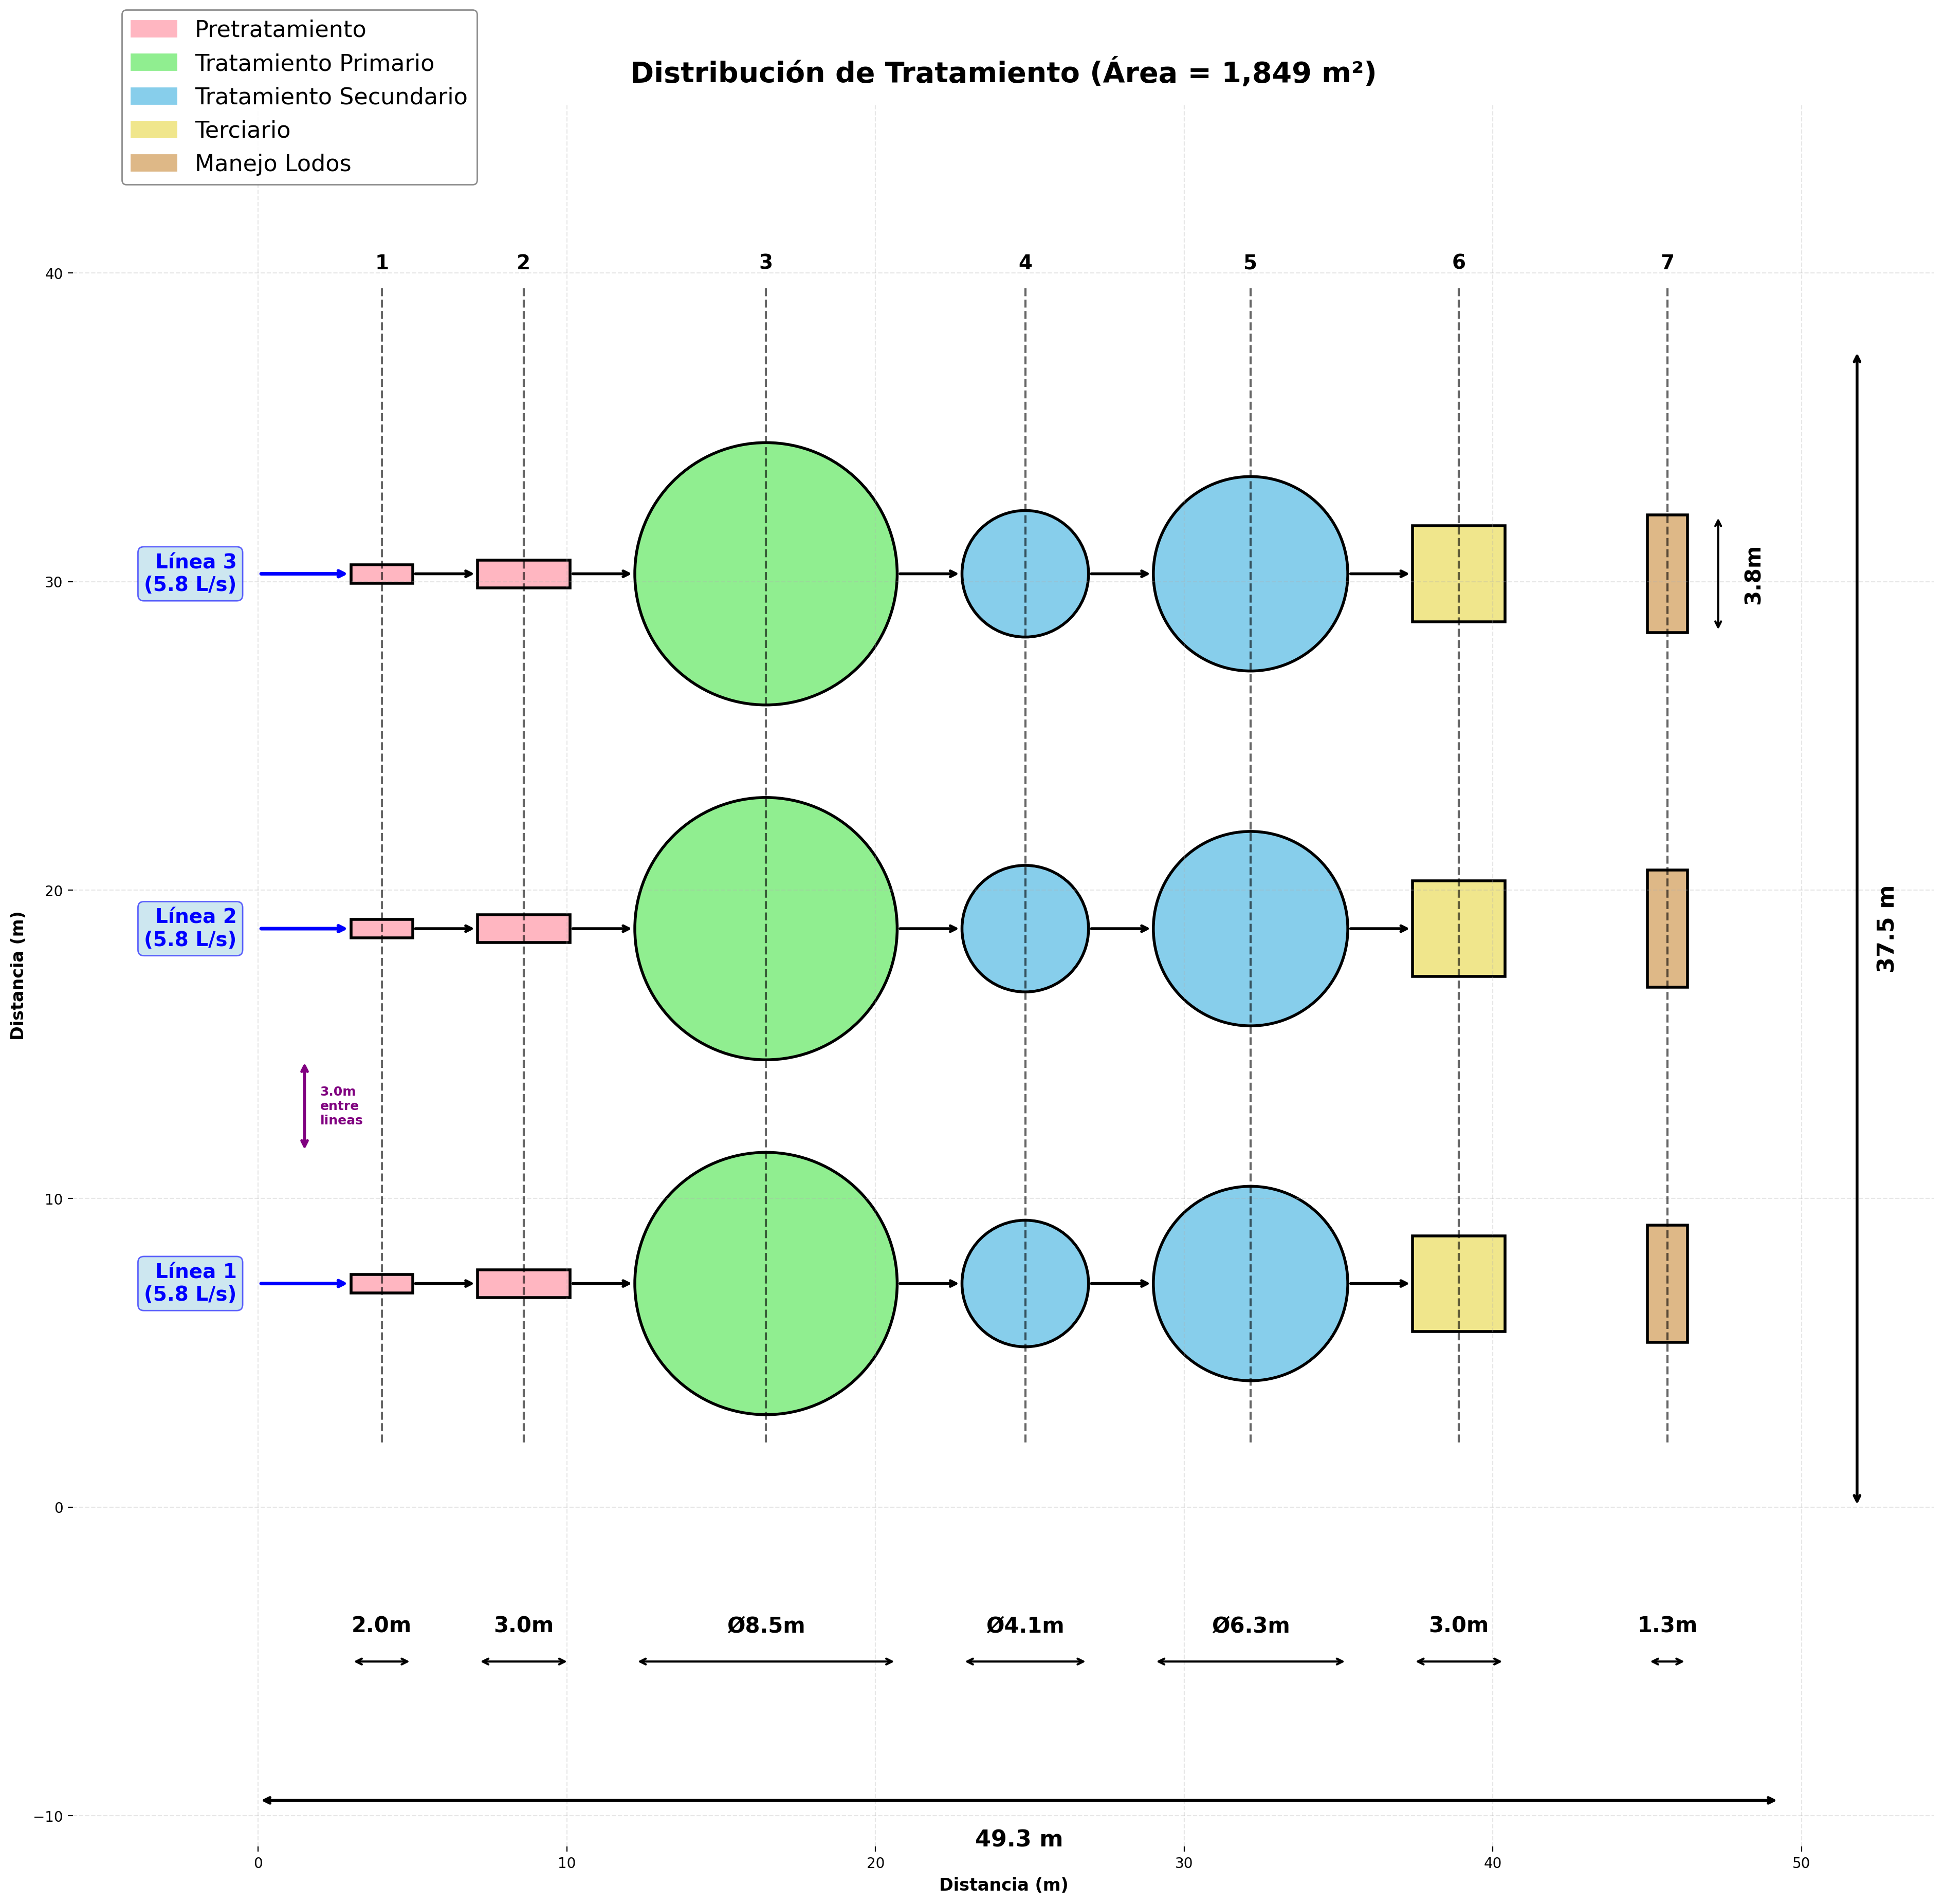
\includegraphics[width=0.8\linewidth]{resultados/_temp_layouts/Layout_t4_uasb_taf_sed_cloro_3lineas.png}
\end{column}
\begin{column}{0.48\textwidth}
\centering
\textbf{T8 (ABR-RAP + TAF + Sed)}\\
2,780~m\textsuperscript{2}
\vspace{2pt}

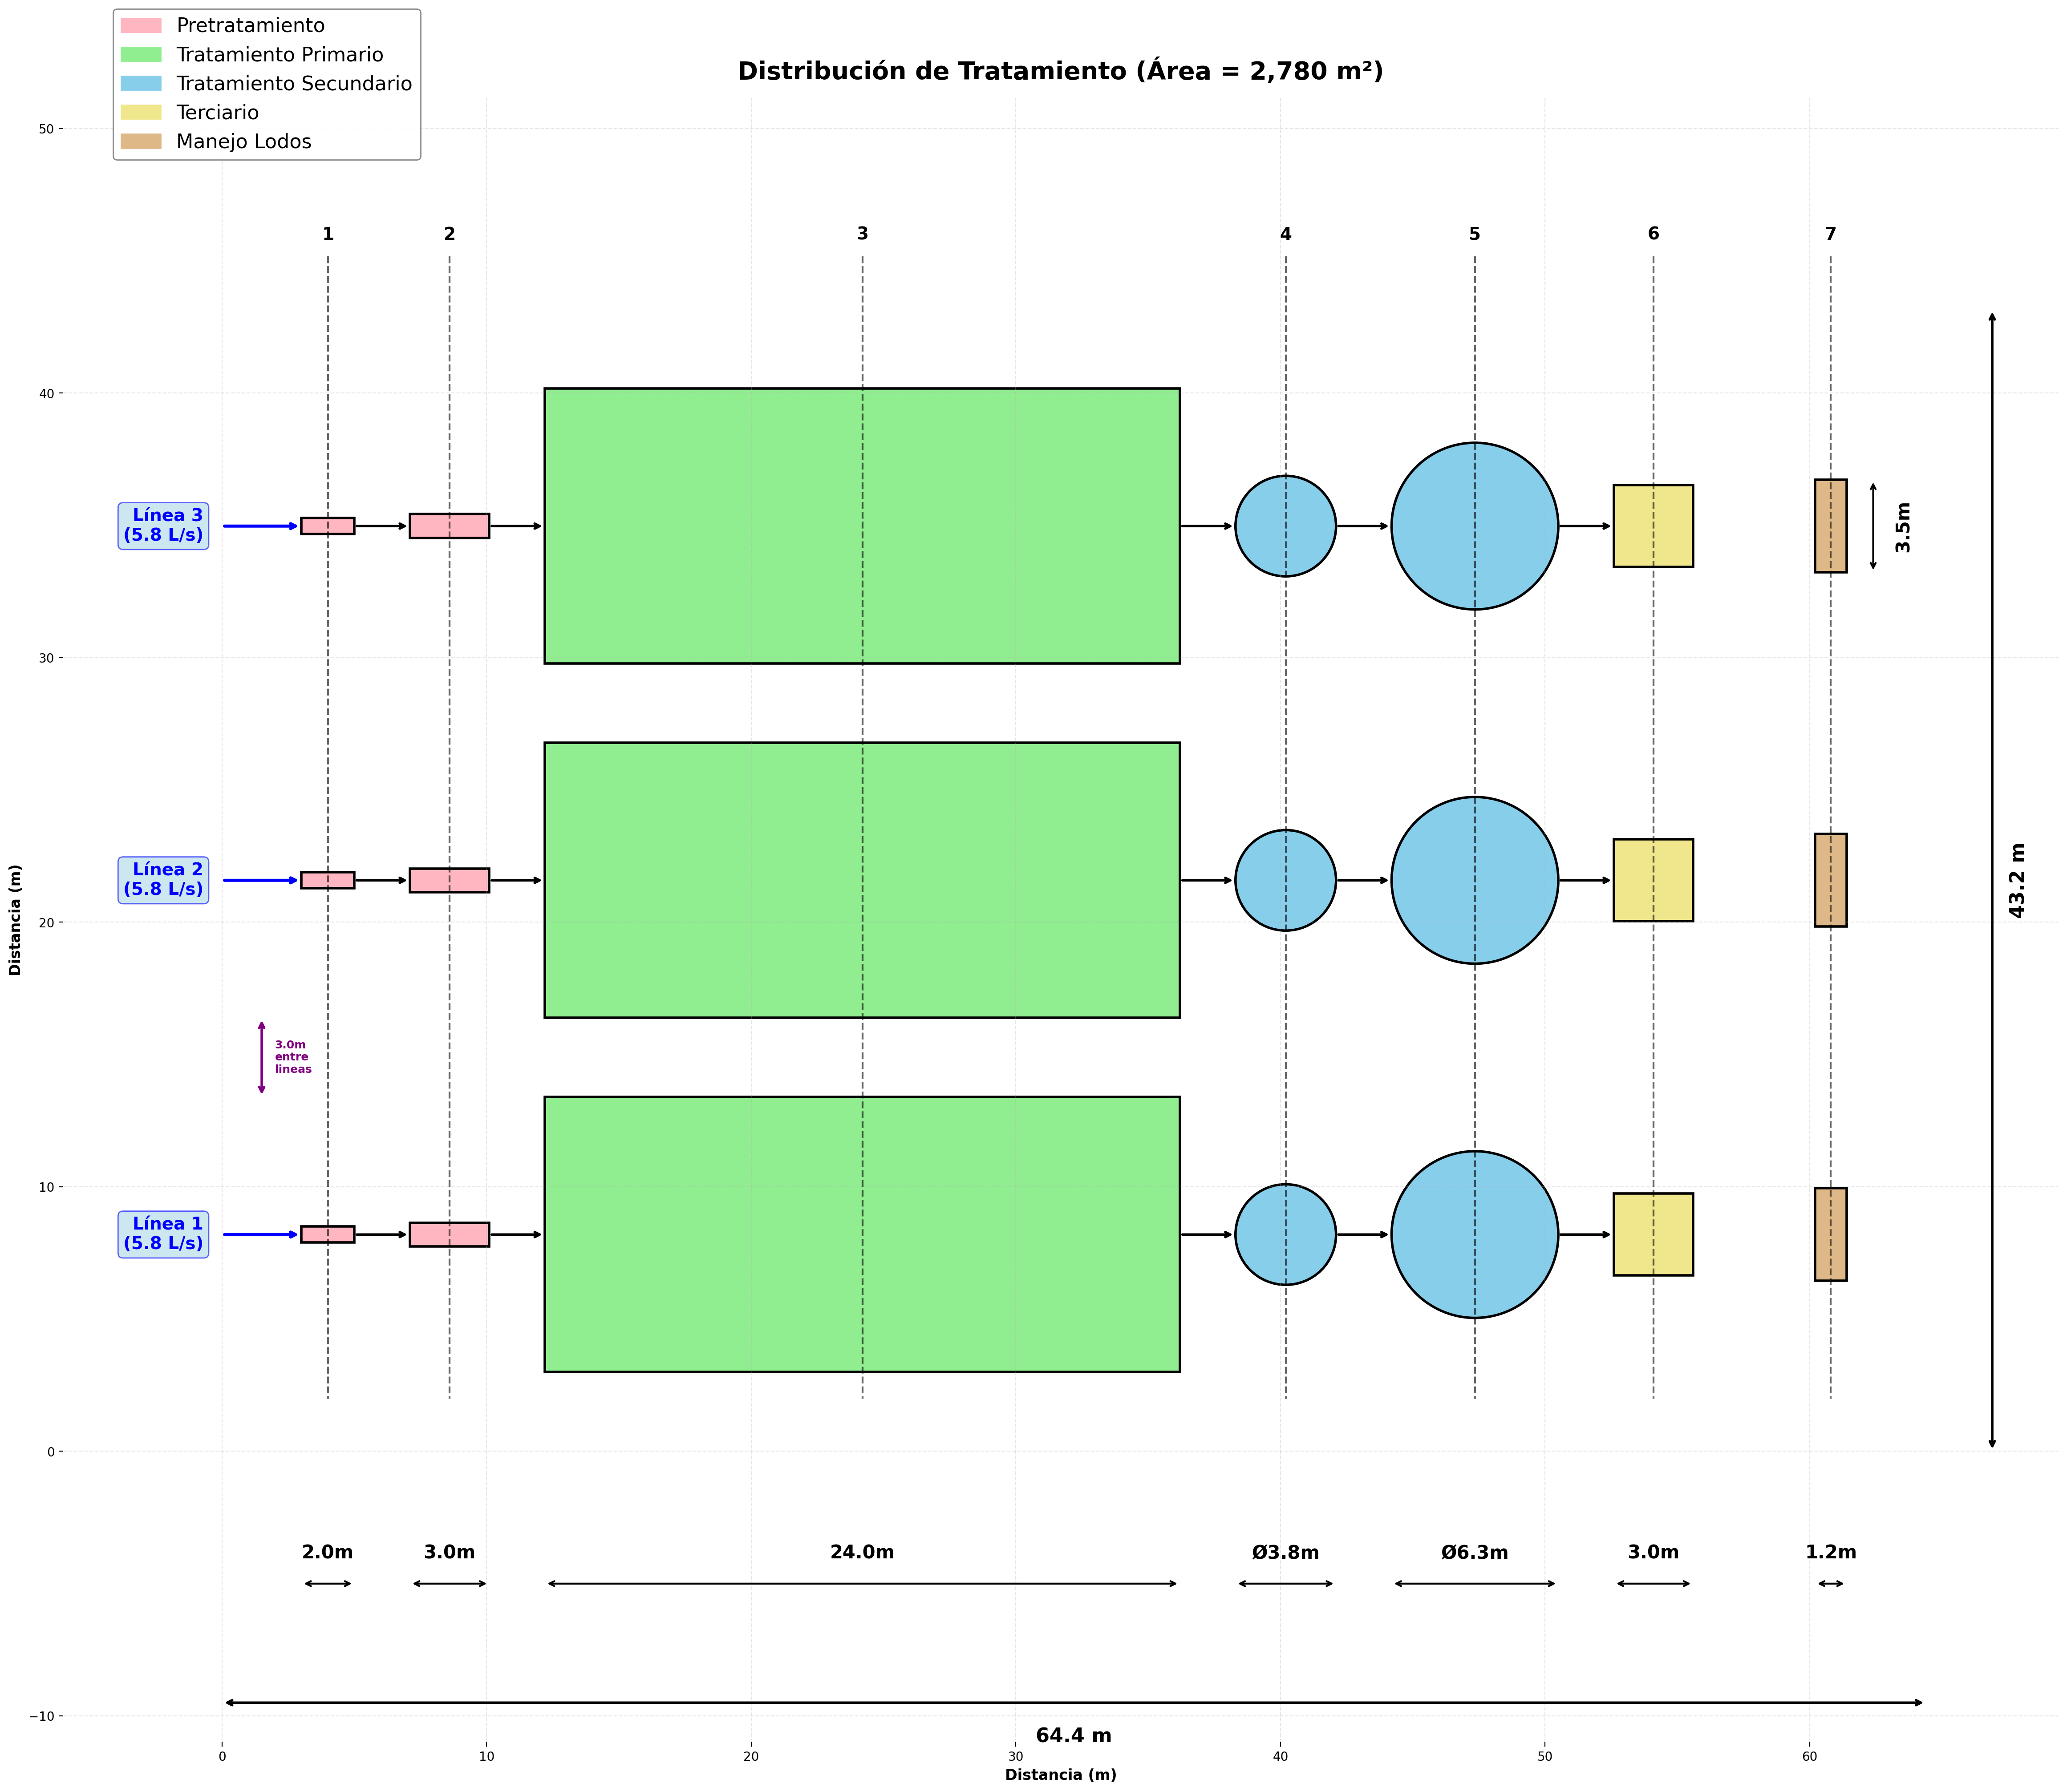
\includegraphics[width=0.90\linewidth]{resultados/_temp_layouts/Layout_t8_abr_taf_sed_cloro_3lineas.png}
\end{column}
\end{columns}
\end{frame}

% ========================================================================
% DIAPO 12.5: AREA TOTAL DEL PREDIO (T4)
% ========================================================================
\begin{frame}
\frametitle{\'{A}rea total del predio: desglose complementario (T4)}
\begin{columns}[T]
\begin{column}{0.55\textwidth}
\scriptsize
\renewcommand{\arraystretch}{1.0}
\begin{tabular}{p{3.4cm}p{3.4cm}r}
\toprule
\textbf{\'{A}rea} & \textbf{Descripci\'{o}n} & \textbf{m\textsuperscript{2}} \\
\midrule
Zona de amortiguaci\'{o}n & Perimetral alrededor de unidades (2--3~m) & 370 \\
Bodega de qu\'{i}micos & Almacenamiento de hipoclorito y productos & 22 \\
Laboratorio/control & An\'{a}lisis de calidad del agua & 33 \\
Caseta de operaci\'{o}n & Control, panel, escritorio, ba\~{n}o & 28 \\
\'{A}rea de lavado & Limpieza de equipos y herramientas & 18 \\
Estacionamiento & Veh\'{i}culos del personal y visitantes & 102 \\
Zona de camiones & Acceso de cisterna/retiro de lodo & 120 \\
Caminos internos & Circulaci\'{o}n vehicular y peatonal & 185 \\
Acceso principal & Entrada, port\'{o}n y caseta de guardia & 46 \\
Bodega general & Herramientas, repuestos, EPP & 33 \\
Zona carga de lodos & Carga/descarga de lodo deshidratado & 46 \\
\'{A}rea verde/buffer & Separaci\'{o}n de l\'{i}mites, revegetaci\'{o}n & 473 \\
\bottomrule
\end{tabular}
\end{column}
\begin{column}{0.43\textwidth}
\footnotesize
\textbf{C\'{a}lculo del \'{a}rea total estimada}\\[4pt]
\scriptsize
Para T4 ($A_{\text{tratamiento}} = 1\,849$~m\textsuperscript{2}):

\vspace{6pt}
\[
A_{\text{total}} = \frac{A_{\text{trat.}} + A_{\text{amort.}} + A_{\text{compl.}}}{1 - 0{,}15}
\]

\vspace{4pt}
\begin{align*}
A_{\text{tratamiento}} &= 1\,849~\text{m}^2 \\
A_{\text{amortiguaci\'{o}n}} &= 370~\text{m}^2~(20\%) \\
A_{\text{complementarias}} &= 462~\text{m}^2
\end{align*}

\vspace{4pt}
\[
A_{\text{total}} \approx \frac{1\,849 + 370 + 462}{0{,}85} \approx \mathbf{3\,154~m^2} \approx \mathbf{0{,}32~ha}
\]

\vspace{6pt}
\scriptsize
\textit{T8 (ABR-RAP + TAF + Sed) escala proporcionalmente a $\sim$4\,750~m\textsuperscript{2} ($\sim$0{,}48~ha) por su mayor \'{a}rea de tratamiento (2\,780~m\textsuperscript{2}).}
\end{column}
\end{columns}
\end{frame}

% ========================================================================
% DIAPO 12.7: COMPARACION DE CAPEX
% ========================================================================
\begin{frame}
\frametitle{Comparaci\'{o}n de inversi\'{o}n inicial (CAPEX)}
\centering
\footnotesize
\renewcommand{\arraystretch}{1.1}
\begin{tabular}{lccc}
\toprule
\textbf{Concepto} & \textbf{Lodos act.} & \textbf{T4} & \textbf{T8} \\
\midrule
Civil + estructuras & \$500--800K & \$350--550K & \$450--700K \\
Electromec\'{a}nico & \$700K--1.1M & \$150--250K & \$180--300K \\
Laboratorio + SCADA & \$150--200K & \$30--50K & \$30--50K \\
Instalaci\'{o}n y puesta en marcha & \$150--250K & \$70--100K & \$90--130K \\
\midrule
\textbf{Total estimado} & \textbf{\$1.4--2.2M} & \textbf{\$600--900K} & \textbf{\$750K--1.1M} \\
\bottomrule
\end{tabular}

\vspace{4pt}
\scriptsize
\textit{Valores referenciales para una PTAR de 1\,500~m$^3$/d en contexto insular. La mayor diferencia est\'{a} en el equipamiento electromec\'{a}nico.}

\vspace{8pt}
\begin{columns}[T]
\begin{column}{0.48\textwidth}
\footnotesize
\textbf{Implicaci\'{o}nes de lodos activados en una linea}\\[2pt]
\scriptsize
\begin{itemize}
\scriptsize
\item requieren repuestos dif\'{i}ciles de conseguir en Gal\'{a}pagos,
\item necesitan t\'{e}cnicos especializados,
\item deprecian r\'{a}pidamente en ambientes salinos.
\item cualquier operacion requiere parar la ptar
\end{itemize}
\end{column}
\begin{column}{0.48\textwidth}
\footnotesize
\textbf{Implicaciones de T4 y T8}\\[2pt]
\scriptsize
Reducen sustancialmente esa exposici\'{o}n al minimizar la mecanizaci\'{o}n cr\'{i}tica y distribuir la funci\'{o}n en unidades m\'{a}s simples y redundantes.
\end{column}
\end{columns}
\end{frame}

% ========================================================================
% DIAPO 13: TESIS TECNICA CENTRAL
% ========================================================================
\begin{frame}
\frametitle{Tesis t\'{e}cnica central}
\begin{columns}[T]
\begin{column}{0.55\textwidth}
\footnotesize
\textbf{Contextualisacion de la alternativa de  lodos activados frente a las restricciones insulares}\\[4pt]

\scriptsize
\begin{itemize}
\item \textbf{Alta dependencia energ\'{e}tica:} aireaci\'{o}n forzada continua ($\sim$0.5~kWh/m$^3$) en una isla con energ\'{i}a costosa.
\item \textbf{Control operativo exigente:} requiere personal calificado, laboratorio y ensayos de jarras disponibles de forma sostenida.
\item \textbf{Sensibilidad a fallas:} sin redundancia ni l\'{i}neas de respaldo, una parada de blower o dosificaci\'{o}n compromete el efluente inmediatamente.
\item \textbf{Log\'{i}stica compleja:} repuestos, qu\'{i}micos y consumibles deben traerse desde el continente.
\item \textbf{Continuidad del servicio:} el arranque biol\'{o}gico tras paradas implica semanas de inestabilidad.
\end{itemize}
\end{column}
\begin{column}{0.43\textwidth}
\footnotesize
\textbf{Ventajas  de T4 y T8}\\[4pt]
\scriptsize


\vspace{4pt}
\renewcommand{\arraystretch}{1.1}
\begin{tabular}{p{3.2cm}c}
\toprule
Criterio & T4 / T8 \\
\midrule
Calidad de efluente & Cumple \\
Dependencia energ\'{e}tica & Baja \\
Complejidad operativa & Baja-media \\
Redundancia arquitect\'{o}nica & S\'{i} (3 l\'{i}neas) \\
Robustez insular & Alta \\
\bottomrule
\end{tabular}

\vspace{4pt}
\scriptsize
\textit{Robustez bajo restricciones  de operaci\'{o}n, mantenimiento y log\'{i}stica en Gal\'{a}pagos.}
\end{column}
\end{columns}
\end{frame}

% ========================================================================
% DIAPO 14: RECOMENDACION + LIMITACIONES
% ========================================================================
\begin{frame}
\frametitle{Conclusiones y condiciones de aplicaci\'{o}n}
\begin{columns}[T]
\begin{column}{0.50\textwidth}
\textbf{Alternativa T4: UASB + TAF + Sed. secundario}\\[4pt]
\small
Menor \'{a}rea (1\,849~m\textsuperscript{2}), efluente DBO\textsubscript{5} = 11.8~mg/L. Adecuada cuando el terreno disponible es el factor cr\'{i}tico y la gesti\'{o}n de lodos puede resolverse con mayor frecuencia de extracci\'{o}n (28.1~kg SS/d).

\vspace{8pt}
\textbf{Alternativa T8: ABR-RAP + TAF + Sed. secundario}\\[4pt]
\small
Mayor \'{a}rea (2\,780~m\textsuperscript{2}), efluente DBO\textsubscript{5} = 9.8~mg/L, producci\'{o}n de lodos reducida a la mitad (14.7~kg SS/d) e incorpora remocci\'{o}n biol\'{o}gica de f\'{o}sforo. Preferible cuando el cuerpo receptor tiene restricciones de nutrientes o cuando la disposici\'{o}n de lodos es log\'{i}sticamente compleja.
\end{column}
\begin{column}{0.48\textwidth}
\textbf{Comparaci\'{o}n con la propuesta con lodos activados}\\[4pt]
\footnotesize
\begin{tabular}{p{2.6cm}p{3.6cm}}
\toprule
Criterio & Propuesta con lodos activados \\
\midrule
Complejidad mec. & Alta (aireaci\'{o}n, dosificaci\'{o}n, retorno) \\
OPEX energ\'{e}tico & Alto ($\sim$0.5~kWh/m\textsuperscript{3}) \\
Dependencia log\'{i}stica & Alta (repuestos, qu\'{i}micos, laboratorio) \\
Redundancia & Ninguna (1 l\'{i}nea) \\
Encadenamiento & Incompleto en la configuraci\'{o}n actual \\
\bottomrule
\end{tabular}
\vspace{6pt}

\footnotesize
\textbf{Limitaciones del an\'{a}lisis:} los scores se basan en par\'{a}metros de dise\~{n}o est\'{a}ndar bajo las mismas condiciones de contorno. Los valores de OPEX energ\'{e}tico son estimativos.
\end{column}
\end{columns}
\end{frame}

\end{document}
